
%------------------------------------------------

\section{Exponential from uniform}
\label{exer:expo_from_uniform}

\subsection{Generate exponential variables from uniform}

\begin{enumerate}
	\item Generate $10^{6}$ values of the variable $t$, uniformly distributed in $[0, \Delta t = 10^{3}]$.
	\item Sort the list of generated values.
	\item Compute the interval $\delta t_{i} = t_{i} - t_{i - 1}$.
	\item Plot the distribution of $\delta t_{i}$ (as a histogram).
	\item Fit it with an exponential. 
		\marginnote{Does it work? Do you get back the input parameters?}
\end{enumerate}

\subsection{Hints for the solution}

Fit the histogram with the following function:

\begin{equation}
	f(\delta t) = n \cdot \lambda_{1} \cdot w_{t} \cdot \mathrm{e}^{- \lambda_{2} \cdot \delta t}
\end{equation}

where: $n = 10^{6}$ (fixed value) and $w_{t} = $ bin width (fixed).

At this point, we need to make sure that the fit outputs the same values for $\lambda_{1}$ and $\lambda_{2}$.

Alternatively, we can fit with:

\begin{equation}
	f(\delta t) = n \cdot \lambda \cdot w_{t} \cdot \mathrm{e}^{- \lambda \cdot \delta t}
\end{equation}

but leaving $n$ a free parameter.

In this case, the fit should return $n = 10^{6}$.

(Figure~\ref{fig:expo_from_uniform})

\begin{figure}
	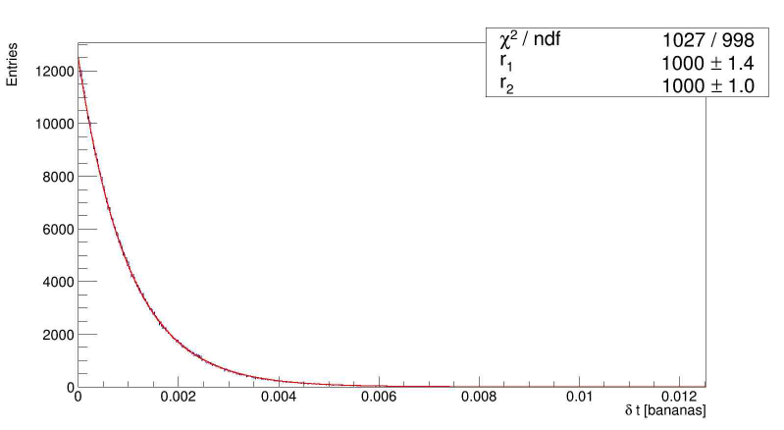
\includegraphics{exercise/expo_from_uniform.png}
	\caption[Exponential from uniform.][6pt]{Exponential from uniform.}
	\label{fig:expo_from_uniform}
\end{figure}

($\hookleftarrow$ \ref{subsec:expo_distr})
